% !TeX spellcheck = en_GB
\documentclass[main.tex]{subfiles}

\begin{document}
\chapter{Methods}
\lhead{Methods}
\label{chap:methods}

\section{Benchmarking Existing Named Entity Recognition}
\subsection{Evaluation of NER}
\label{subsec:nereval}
\subsection{Fine-tuning English LUKE}
Yamada et al. benchmark LUKE, on Named Entity Recognition using the CoNLL-2003 dataset \cite{yamada2020luke}.

Reproduction of these results were attempted by obtaining the pretrained LUKE models from Yamada et al.'s software repository.
The same hyper-parameters as Yamada et al. were used and are shown along with and technical details in Table~\ref{tab:params}.

The finetuning procedure was repeated five times for each of the two released LUKE models, called \emph{large} and \emph{base}, to examine variability in the downstream training.
%%% Horrible footnote manipulation - it works, dont touch it! %%%
\addtocounter{footnote}{1}
\footnotetext{\label{foot:fnt}
    The pre-trained models were downloaded on 17/02-2021 from the LUKE software repository:
    \url{https://github.com/studio-ousia/luke/tree/6feefe657d97d2f847ace87f61f23b705f75d2aa\#released-models} 
} 
\begin{table}[H]
    \centering
%    TODO The number of parameters is clearly mixed up. Is the learning rate too?
    \begin{tabular}{l|rr}
        Pre-trained model
                                    & LUKE large \textsuperscript{\ref{foot:fnt}}\
                                                & LUKE base\textsuperscript{\ref{foot:fnt}}\\\hline
        Pre-trained model parameters & $253\ctp 6$ & $483\ctp 6$\\
        Pre-trained model entity vocabulary & $500\ctp3$ & $500\ctp3$\\
        Learning rate               & $10^{-5}$ & $5\ctp{-5}$\\
        Effective batch size        & 16 & 16\\
        Gradient accumulation steps & 2 & 2\\
        Numeric precision           & \multicolumn{2}{l}{Mixed FP16/FP32 (Nvidia APEX)}\\
        Training code               & \multicolumn{2}{l}{PyTorch-based \code{luke}-repository \protect\footnotemark}\\
        Software version            & \multicolumn{2}{l}{Python 3.6, PyTorch 1.2}
    \end{tabular}
    \label{tab:params}
\end{table}

\footnotetext{
    The repository \url{github.com/studio-ousia/luke} was cloned at commit-SHA \code{6feefe6}, installed and used for the fine-tuning.
}
\subsection{Off-the-shelf, Danish models}
\label{sec:exidan}
A number of Danish NER models that are publily available and usable by NLP practitioners were collected and evaluated on the testing datasets of the three Danish NER annotations considered in Section \ref{subsec:daNERdata}:
DaNE, Plank and Wiki-ANN.

Most of the models were found through DaNLP \cite{danlp2021} and a number of them are introduced in Section \ref{sec:nlpda}.

\setlist{itemsep=.5em}
\begin{itemize}
    \item \textbf{DaNLP da-BERT}: The daBERT model \cite{botxo2019dabert} finetuned for NER on DaNE by DaNLP.
    \item \textbf{NERDA m-BERT}: The multilingual BERT base released by the original Google Research BERT team \cite{devlin2019bert} finetuned by NERDA \cite{kjeldgaard2020nerda} on DaNE.
    \item \textbf{NERDA Ælæctra}: The transformer Ælæctra, released by Malte Højmark-Bertelsen, \cite{bertelsen2020lctra} finetuned by NERDA on DaNE.
    \item \textbf{DaCy}: An adaption of version 3 of the SpaCy framework \cite{honnibal2020spacy} to Danish by Kenneth Enevoldsen including finetuning of on DaNE \cite{enevoldsen2020dacy}.
        Both the medium and large versions are benchmarked, using the base and large multilingual RoBERTa model, respectively.
        This 2021 model, large version, is the currently reported state of the art.
    \item \textbf{DaNLP spaCy}: SpaCy, version 2, adapted to Danish by DaNLP and finetuned on DaNE.
    \item \textbf{DaNLP Flair}: The Flair framework \cite{akbik2019flair} also adapted to Danish by DaNLP and finetuned on DaNE.
    \item \textbf{Polyglot}: A NLP framework supporting a wide range of tasks in many languages including NER in 40 different languages.
        The NER model is finetuned using automatic, language-agnostic annotations generated from Wikipedia and Freebase link structures \cite{rfou2015polyglot}.
    \item \textbf{daner (DKIE Stanford CRF)}: An application of the Stanford CoreNLP Conditional Random Field (CRF) NER classifier \cite{manning2014corenlp} released Leon Derczynski asa part of the DKIE project \cite{derc2014dkie}.
    The model was trained on NER annotations produced at ITU on the Danish Dependency Treebank (DDT) corpus \cite{kromann2003ddt}.
    The released Java-based NER tool is called \code{daner}\footnotemark.
\footnotetext{
    The repository is at \url{github.com/ITUnlp/daner}
}
\end{itemize}
\setlist{noitemsep}
\noindent
The weights of all these finished NER models were downloaded and evaluated in accordance with Section \ref{subsec:nereval}.
The code for performing inference for all the models on the three datasets and measuring the F1 scores can be found in module \code{reproduction.danish\_ner} in the DaLUKE repository\footnotemark.
The reproduction was performed using Python version 3.7.10 and the dependency versions defined in the requirements of DaNLP and NERDA.
\footnotetext{
    The reproduction code is available here:
    \url{github.com/peleiden/daluke/tree/master/reproduction/danish_ner}.
}
\section{DaLUKE}

\subsection{Pretraining Methodology and Hyperparameters}%
\label{sub:dalpre}
\begin{enumerate}
    \item Måske mere detaljeret beskrivelse af arkitektur -- og illustration?
    \item Vis LR her
    \item Det her afsnit skal være lidt mere detaljeret IMO: Fortæl kort om vores optimeringsmetode + loss + gradientakkulumation
    \item Top $K$
\end{enumerate}
DaLUKE's pretraining largely follows LUKE's with some differences:
\begin{itemize}
    \item The entity-augmented Danish Wikipedia described in section \ref{subsec:entaug} is used.
    \item Entity-aware self-attention is used for the pretraining.
    \item Weights are initialized from da-BERT.
    All four attention matrices described in section \ref{subsubsec:entityaware} are initialized to the same attention matrix in da-BERT.
    \item The full entity vocabulary is used.
\end{itemize}
Due to the memory intensive nature of the transformer architecture, we follow Yamada et al. and use gradient accumulation over multiple subbatches within each batch.

As with LUKE, the cross entropy loss is calculated using equation \ref{eq:crossentropyloss} for each classification task, with the only difference being that the final loss is the average rather than the sum of the individual task losses.
This effectively just scales the loss and has no effect on the learning if the learning rate is adjusted accordingly.

The hyperparameters used for pretraining are shown in table \ref{tab:pretrain-hyper}.
\begin{table}[H]
    \centering
    \begin{tabular}{l|r}
        Parameter  &    Value\\\hline
        Epochs     & 150\\
        Batch size &    4080\\
        Peak learning rate & $3\ctp{-4}$\\
        LR warmup steps prop. & $ 6\pro $\\
        Mask prob. for words & $ 15\pro $\\
        Mask prob. for entities & $ 15\pro $\\
        Dropout & $ 0.1 $\\
        Weight decay & $ 0.01 $\\
        AdamW $ \beta_1 $ & $ 0.9 $\\
        AdamW $ \beta_2 $ & $ 0.999 $\\
        AdamW $ \epsilon $ & $ 10^{-6} $
    \end{tabular}
    \caption{Hyperparameters for DaLUKE pretraining.}\label{tab:pretrain-hyper}
\end{table}\noindent

\paragraph{Learning rate}
LUKE follows BERT and increases its learning rate linearly from 0 to the peak learning rate followed by a linear decrease to 0 for the rest of the learning rate - the slanted triangle learning rate (STLR). \cite{devlin2019bert} \cite{yamada2020luke} \cite{howardruder2018universal}

For pretraining, DaLUKE also employs linear warmup for the first 6\pro\ of parameter updates, after which it decreases polynomially with a power of $ \sqrt{3} $ and a final learning rate of one tenth the peak learning rate.
This results in a more aggressive decrease in learning rate after the warmup period but a slightly higher learning rate in the final steps compared to STLR.
The learning rate development is shown on figure \ref{fig:lr}.
\begin{figure}[H]
    \centering
    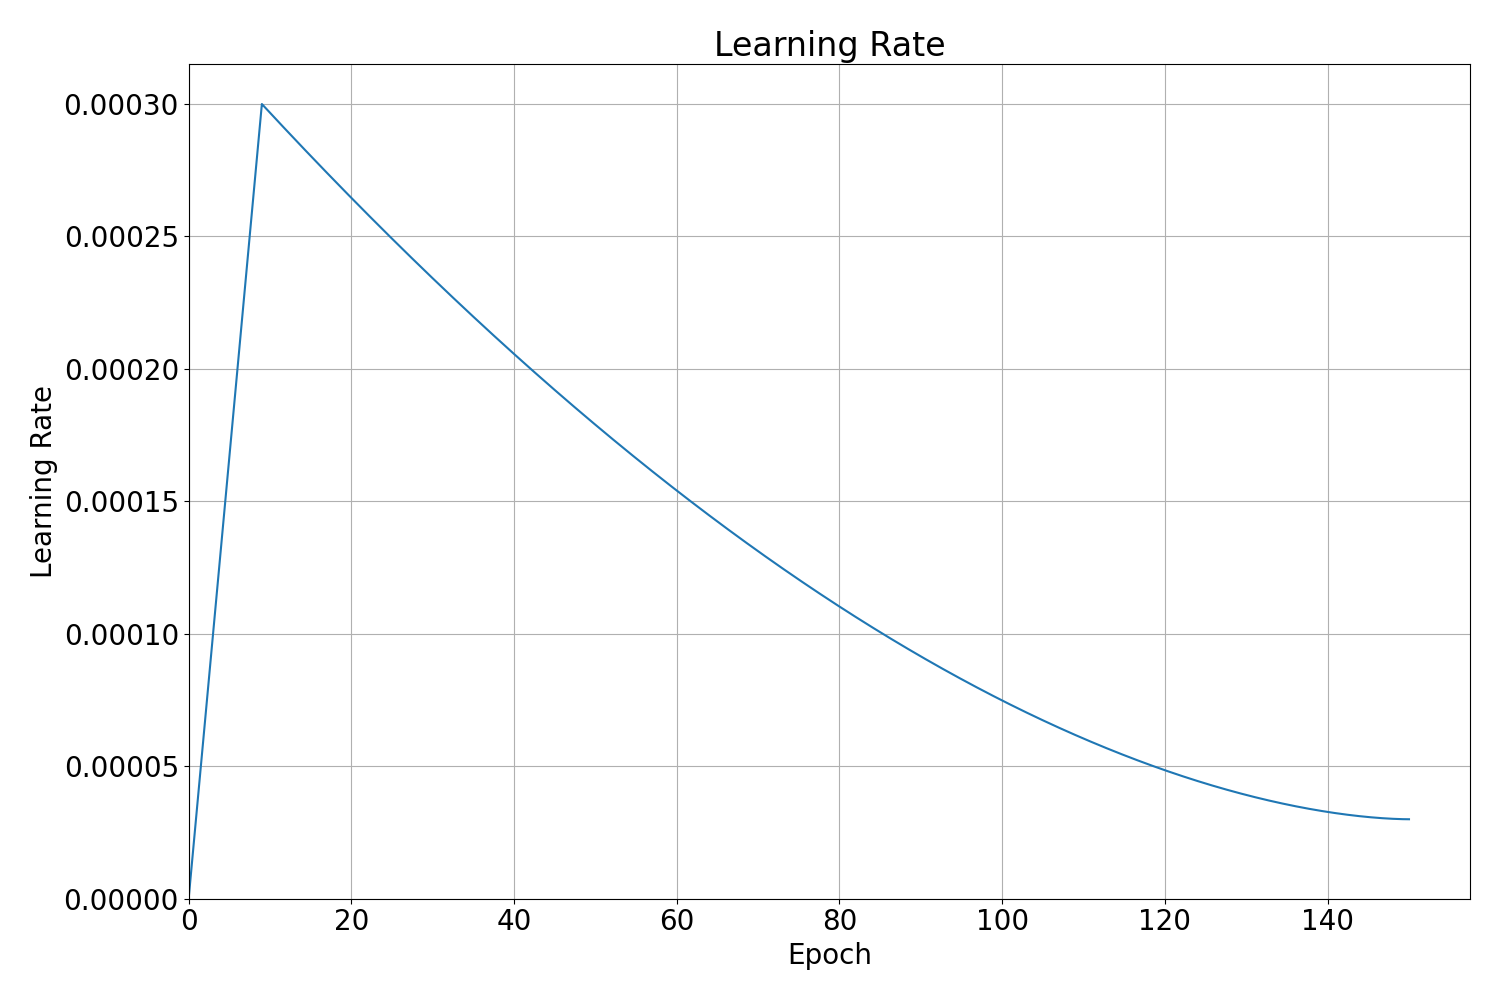
\includegraphics[width=.7\textwidth]{lr}
    \caption{Learning rate during the pretraining.}
    \label{fig:lr}
\end{figure}\noindent

\paragraph{Accuracy measures}
In order to measure the performance of the pretraining model, the accuracy of word and entity predictions are calculated throughout the training.
Due to the size of the classification problem, especially regarding entities, top $ k $ accuracies are calculated for each - that is, if the true token was among the $ k $ tokens given the highest probability by the model.
Top 1, 3, 5, and 10 accuracies are calculated for both the masked word and masked entity task using every example that the model trains on, while top 25 and 50 are calculated using one twentieth of examples for computational efficiency.

\subsection{Fine-tuning DaLUKE for Named Entity Recognition}%
\label{sub:finetune-ner}
The fine-tuning of DaLUKE largely follows that of LUKE, described in section \ref{sec:LUKE}.
Fine-tuning is performed on the three Danish NER datasets DaNE, Plank, and Wiki-ANN.
Unlike Wiki-ANN, DaNE and Plank both contain MISC annotations.
Existing models are inconsistent in whether or not they train and/or evaluate using MISC on these datasets (see table \ref{tab:daNERdata}).
For this reason, we always train using MISC but evaluate both with and without it.
When evaluating without MISC, MISC predictions are treated as non-entity predictions.

%TODO Hvad står dev. for? Development?
The hyperparameters listed in table \ref{tab:finetune-hyper} were used for training.
After each epoch, the model is evaluated on the dev. part of the data-set.
If it gets a better score than the hitherto best checkpoint, the checkpoint is overwritten.
The best checkpoint of the model was used for evaluation on the test set.
\begin{enumerate}
    \item Til hovedeksperimentet bruger vi ikke faste hyperparametre, men søger i hyperparam-optimering.
\end{enumerate}
\begin{table}[H]
    %    TODO Make these up to date
    \centering
    \begin{tabular}{l|r}
        Parameter  &    Value\\\hline
        Epochs     & 15\\
        Batch size &    16\\
        Peak learning rate & $2\ctp{-5}$\\
        LR warmup steps prop. & $ 6\pro $\\
        Dropout (pretrained model) & $ 0.1 $\\
        Dropout (final, linear layer) & $ 0.05 $\\
        Weight decay & $ 0.01 $\\
        AdamW $ \beta_1 $ & $ 0.9 $\\
        AdamW $ \beta_2 $ & $ 0.98 $\\
        AdamW $ \epsilon $ & $ 10^{-6} $
    \end{tabular}
    \caption{Hyperparameters for DaLUKE fine-tuning.}\label{tab:finetune-hyper}
\end{table}\noindent

\paragraph{Learning rate}
Unlike in the pretraining, we do as Yamada et al. and use a slanted triangle learning rate \cite{yamada2020luke}.
Howard and Ruder have also shown that the slanted triangle approach for fine-tuning tasks improve results over a linear decaying learning rates without warmup \cite{howardruder2018universal}.

\paragraph{Loss}
Due to the nature of the $ n $-grams, only very few spans actually cover entities, making the O class dominate the dataset.
For instance, in the training set of DaNE, the O class accounts for 99.3\pro\ of spans.
Furthermore, the actual entities themselves are not perfectly balanced as all things should be.
This naturally poses the question: Will class-weighted cross entropy loss perform better?

This is investigated in section \ref{sec:finetuning-exp}.
The class-weighted loss $ l_w $ is calculated similarly to the unweighted loss in equation \eqref{eq:crossentropyloss}:
\begin{equation}\label{eq:w-crossentropyloss}
    l_w = \frac{1}{\sum_{j=1}^{C} w_j}
    \sum_{i=1}^N w_{c_i} \left(
        -X_{i, c_i} + \log \sum_{j=1}^C \exp X_{i, j}
    \right)
\end{equation}
where $ w_j $ is weight of class $ j $ \cite{pytorchcel}.
There are multiple ways to define the class weights.
Arguably the simplest, and the one used here, is the reciprocal of the number of occurrences of each class in the dataset.

Unless otherwise stated, all fine-tunings presented in the rest of the paper use the non-weighted loss.

\paragraph{Hyperparameter search}

\begin{enumerate}
    \item Hyperparametersøgning for daluke-ner
    \item Vis også resultater
\end{enumerate}
\subsection{Implementation Details and Open Source Software}%
\label{sub:oss}

\subsubsection{Open Source Software Package}
\begin{enumerate}
    \item Minidokumentation
    \item Link til læsmig.md
\end{enumerate}
We publish DaLUKE and all related code under the MIT open source software license \cite{mitlicense}.
All code and documentation is available at \url{https://github.com/peleiden/daluke}.
The pretrained model is available with and without MLM layers at TODO.
The model finetuned on DaNE is available at TODO.
Our software package is \code{pip} installable and runs on Python 3.8 and above.
Simply run `pip install daluke` to install it on your computer.
It allows for using DaLUKE for NER on text files directly from the command line.

\paragraph{Implementation}
Yamada et al. have made their code\footnote{\url{https://github.com/studio-ousia/luke}. Visited June 11, 2021.} freely available under the Apache License 2.0 \cite{apachelicense}.
We highly appreciate this, and our original plan was to use their code and then as necessary fit it to our needs.
However, we quickly ran into a number of issues with this approach:
Getting all dependencies installed with the correct versions proved to be a very challenging task.
To solve this, we forked the repository and updated both Python and several of the dependencies to newer versions, but this in itself required major code rewrites.
When that worked, we started pretraining, which had more mysterious issues:
Training on a single GPU worked, but two GPU's slowed training by a factor of three, and three or more GPU's simply did not work.
Due to limited GPU availability, cryptic error messages, and an almost complete lack of documentation, debugging once again became very challenging.

These reasons compelled us to reimplement the model and training from scratch.
This would also help us understand LUKE better due to being forced to work with all the details of the model and training tasks.
Finally, it would make it much easier to fit the code to our needs, as we would have a much better understanding of the code base.
The forked LUKE repository, available at \code{https://github.com/peleiden/luke}, is used for parts of the data-set preparation, but everything else has been reimplemented.
Our code is inspired from the original LUKE code, but we have made efforts to make it more approachable by making the code more readable and better structured and especially by increasing the amount of documentation.

Rewriting code bases always carries a risk of introducing bugs.
Despite borrowing heavily from Yamada et al., we did introduce a number of bugs in the code that had to be fixed, forcing multiple restarts of the training.
These ranged from domain specific such as accidentally leaving category pages in the entity vocabulary to classical ones such as copying pointers instead of the memory stored at them.
In that regard, using the original code would be safer, as this has been proven to work.
However, the original code is also not error free.
For instance, we discovered a bug in the masking where the unmasking and random word replacements would either be done or not done for an entire sequence, rather than being probabilistic for every masked sub-word token.
We have opened an issue on the LUKE repository that can be followed here.
%TODO Make issue

\subsubsection{Floating Point Precision}
The model is trained using PyTorch Automatic Mixed Precision (AMP) \cite{pytorchamp}, which -- ideally, at least -- should decrease training time with little to no penalty to accuracy \cite{huang2020amp}.
This is partially due to half-precision calculations being simpler, and partially due to the lower memory requirements, allowing larger subbatches and thus better GPU utilization.
However, as figure \ref{fig:runtime} shows, AMP works as intended when training on NVIDIA V100's, but has the opposite effect when training on NVIDIA A100's.

AMP works by automatically casting parts of the model to half precision rather than the usual single precision.
Some layers are more sensitive than others to precision.
For instance, linear layers are always casted to half precision, but the loss is calculated using single precision.
Due to the smaller precision, underflow in the gradients is a risk.
This is handled by scaling up the loss and then scaling down the gradients accordingly.
\cite{pytorchamp}

\subsubsection{Distributed Training and Runtime}
As transformer training requires significant compute, distributing the training over multiple GPU's can yield significant speedups.
Especially given the parallelizable nature of the transformer compared to recurrent neural network variations \cite{vaswani2017att}, training should scale fairly well on multiple GPU's.

The pretraining took roughly a week.
Due to varying GPU availability, varying numbers of A100's and V100's were used for pretraining and the experiments in section \ref{sec:pretrainpls}.
The main pretraining took approximately a week and used 2-4 V100's.
For comparison, Yamada et al. train LUKE using 16 V100's over a period of 30 days. \cite{yamada2020luke}

We measure the time needed to train for one epoch on different cluster configurations.
The results are shown on figure \ref{fig:runtime}.
\begin{figure}[H]
    \centering
    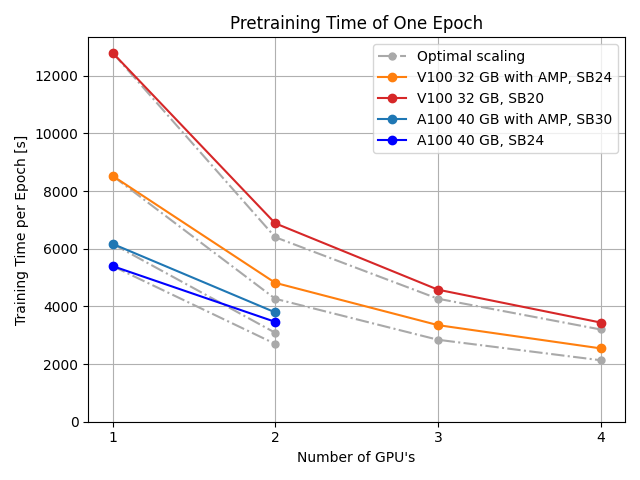
\includegraphics[width=.7\textwidth]{runtime}
    \caption{
        How GPU models, the number of GPU's, and AMP influences pretraining runtime.
        Sub-batch size (SB) is included, as it is important for GPU utilization.
        The measurements were taken with da-BERT weights locked.
        The V100's act mostly as expected with close to optimal scaling and AMP decreasing runtime.
        Surprisingly, however, the A100's, while faster, scale poorly and are slower when using AMP.
        The poor scaling is partially explained by Amdahl's law \cite{klein2011amdahl}: The sequential parts of the code do not get faster along with the GPU and so take up a relatively larger amount of the runtime.
        The A100's also do not have an NVLink bridge unlike the V100's and must therefore communicate over PCIe, which is slower.
        The poor AMP performance, however, is harder to explain.
        According to our cluster specialist, it is caused by different \code{gemm} implementations, but we have not investigated it any further.
        Python 3.8.4 using PyTorch 1.8.1 compiled with CUDA 11.1 was used.
    }
    \label{fig:runtime}
\end{figure}\noindent


\end{document}
